%\subsection{An\'alisis suplementarios}\label{sec:escenario1_supl}
\par Teniendo una gran cantidad de informaci\'on capturada en las distintas redes
que componen este escenario, corresponde quiz\'as hacer un an\'alisis un poco
m\'as profundo sobre las distintas variables que podemos identificar y guardar
durante la etapa de \textit{sniffing}.

\par Estas variables pueden ser muchas. En particular identificamos dos variables,
por ah\'i un tanto inmediatas y no muy complejas, pero no por ello menos importantes
o menos propensas a otorgarnos informaci\'on. Estamos hablando de la parametrizaci\'on
seg\'un el tiempo (cuando fue capturada cierta informaci\'on) y la cantidad (cuanta
informaci\'on).

\par As\'i pues, en un principio resulta interesante para comprender el comportamiento
de las redes ver el vol\'umen de paquetes ARP durante per\'iodos m\'as cortos. Hasta
este momento, en este escenario nos estuvimos concentrando en comprender a toda la
informaci\'on capturada como 2 grandes fuentes de informaci\'on (fuente origen y
fuente destino). Proponemos, entonces, observar que ocurre m\'as granularmente
al comprender a las fuentes de informaci\'on no como un \textit{todo}, sino analizando
que ocurr\'io cada d\'ia de captura.


\subsubsection{Vol\'umen de paquetes ARP por d\'ia/hora}
\par En la figura \ref{fig:arp_por_hora} se pueden observar como
va evolucionando la cantidad de paquetes capturados en per\'iodos de 60 minutos, y a
su vez comparar este comportamiento en los diferentes d\'ias.

\begin{figure*}[!b]
    \begin{tabular}{cc}
        \centering
        \subfloat[\nameref{itm:vlan10}]{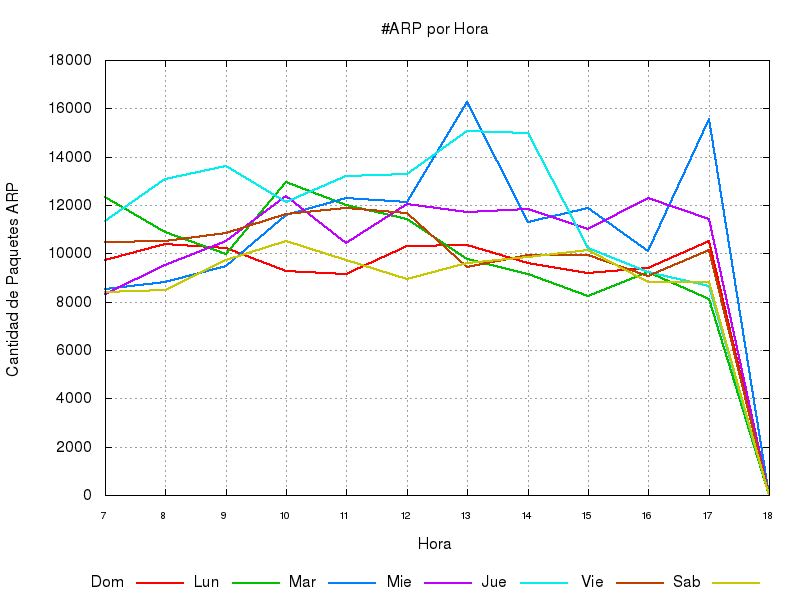
\includegraphics[width=0.5\textwidth]{img/graph/escenario_1/vlan10/vlan10_arp_per_hour_lines}} &
        \subfloat[\nameref{itm:vlan20}]{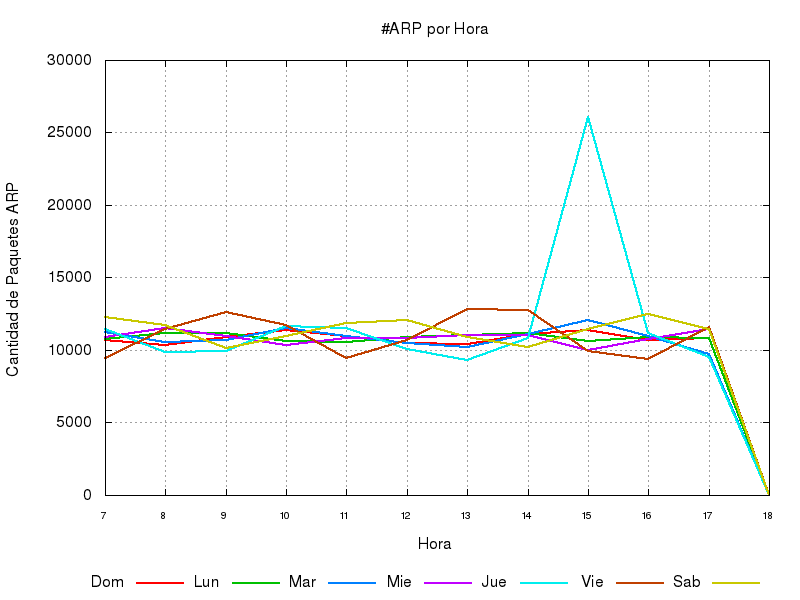
\includegraphics[width=0.5\textwidth]{img/graph/escenario_1/vlan20/vlan20_arp_per_hour_lines}} \\
        \subfloat[\nameref{itm:vlan40}]{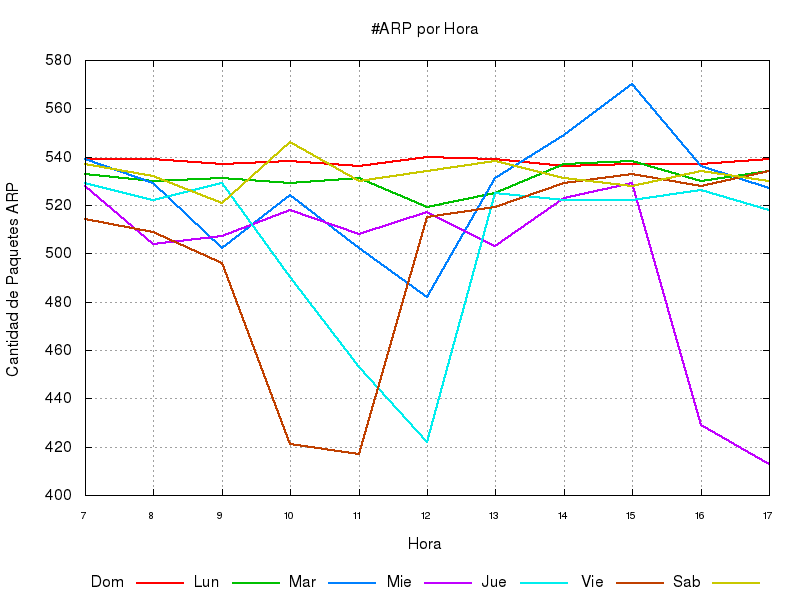
\includegraphics[width=0.5\textwidth]{img/graph/escenario_1/vlan40/vlan40_arp_per_hour_lines}} &
        \subfloat[\nameref{itm:vlan1}]{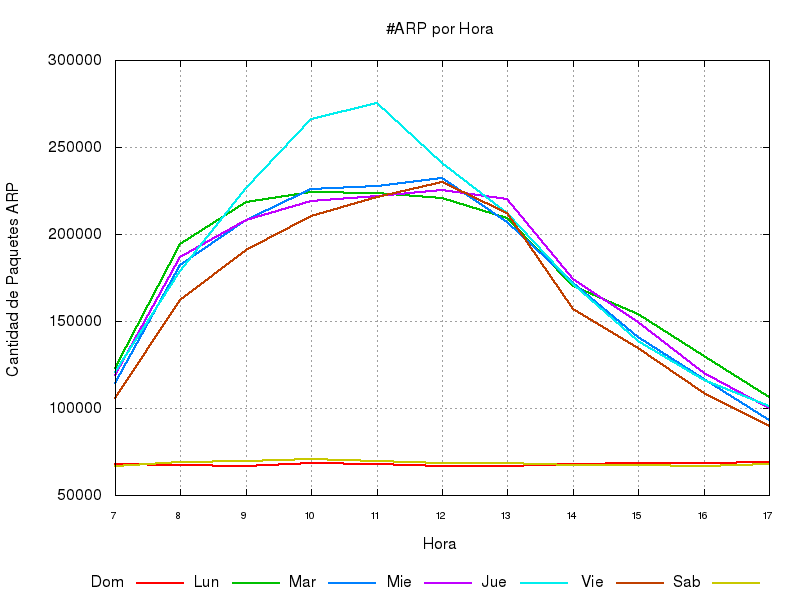
\includegraphics[width=0.5\textwidth]{img/graph/escenario_1/vlan1/vlan1_arp_per_hour_lines}} \\
    \end{tabular}
    \caption{Cantidad de paquetes ARP por hora}
    \label{fig:arp_por_hora}
\end{figure*}

\par Como primer resultado, que claramente salta a primera vista, es que el
comportamiento\footnote{Siempre pensado respecto de los paquetes ARP que se
encuentran en la red.} de las redes es bastante ca\'otico en cuanto a la cantidad
de paquetes por hora y d\'ia.

\par Claramente, el experimento realizado no nos permite decir exactamente que
est\'a ocurriendo en la red, pero si vemos que en el aspecto de como var\'ia
el vol\'umen de estos paquetes (y por lo tanto, una parte importante de la
congesti\'on de la LAN) nos encontramos con tres casos que parec\'ieran
seguir patron, mientras que la red de \nameref{itm:vlan40} pareciese,
\textit{a priori}, no hacerlo

\par Respecto de esto, y con el conocimiento que se tiene de que dispositivos/%
usuarios participan de la red, queda claro que el comportamiento aleatorio de
los usuarios con sus terminales (e incluso con terminales que un d\'ia est\'an
y otro no; o incluso que se conectan a la red en franjas horarias dispares)
tiene un impacto direct en la cantidad de paquetes que circulan en la red. M\'as
interesante, se puede observar que el vol\'umen es claramente m\'as alto en los
alrededores del mediod\'ia (comparando cada d\'ia en su variaci\'on por hora) y
en los d\'ias intermedios de la semana (comparando una misma hora pero en distintos
d\'ias)

\par Este \'ultimo detalle no s\'olo ocurre en la red de \nameref{itm:vlan10},
sino que tambi\'en se puede observar, y mucho m\'as marcado, en la red
\nameref{itm:vlan1}. Se observa aqu\'i que el vol\'umen es muy estable, bajo y
parejo los S\'abados y Domingos, y que durante los d\'ias de la semana se observa
un vol\'umen m\'as grande en la franja horaria de 9 a 14 hs, que luego se reduce
considerablemente hacia el fin de la jornada laboral\footnote{En particular, la
mayor\'ia de los usuarios de las redes observadas utiliza la red entre las 7 y
las 15 hs}. 

\par A pesar de ver este comportamiento similar, debemos aclarar
que los vol\'umenes de ambas redes son claramente distintos. Sin ir m\'as lejos,
en el caso promedio, la red \nameref{itm:vlan1} tiene 20 veces m\'as paquetes ARP
que \nameref{itm:vlan10}. Es decir, podr\'iamos tener una variacia\'on m\'as
grande, nominalmente hablando, dentro de esta red. Pero tomando en cuenta
el vol\'umen total y la cantidad de paquetes, es admitible la comparaci\'on.

\par Algo remarcable de esta similitud reci\'en expuesta, es que la red de
\nameref{itm:vlan1} tiene muchos servidores aparte de usuarios, y si obsevamos
el grafico correspondiente a la red \nameref{itm:vlan20}, veremos un vol\'umen
similar al de la red \nameref{itm:vlan10} y de comportamiento igualmente
dispar\footnote{M\'as all\'a del \textit{outlier} correspondiente a las
15 hs del Jueves. Probablemente hubo alguna instalaci\'on de servidores o
software en los mismos que impactaron en la red.}. Al observar
una red que combina, esperablemente, los comportamientos de estos dos tipos
de redes, nos encontramos con una red que tiene un vol\'umen base seguramente
dependiente de los servidores\footnote{ya que estos no suelen desconectarse y
tienen un comportamiento m\'as estable que las terminales de usuarios}
(claramente observable en las l\'ineas que corresponde nal S\'abado y Domingo)
y luego durante los d\'ias de semana con la afluencia de las terminales de
los empleados, se ve como el vol\'umen se incrementa not\'ablemente.

\par En cuanto a la red de \nameref{itm:vlan40}, simplemente podemos ver
que maneja un vol\'umen que no pareciese seguir un patr\'on respecto
de las horas ni los d\'ias. No s\'olo eso, sino que el vol\'umen que manejan
pareciera ser m\'as estable que en el resto de los casos (mucha menos
variaci\'on de vol\'umen por hora y d\'ia). As\'i pues, podemos determinar
que estos dispositivos (al menos los que se utilizan en esta red, no podr\'iamos
hacer la siguiente aserci\'on para todas las redes de telefon\'ia) hacen un
uso distinguiblemente menor en cuanto a la identificaci\'on de las \textit{MAC}
de los dem\'as. Esto tambi\'en podr\'ia deberse a que la cantidad de dispositivos
conectados es mucho menor y por ah\'i los dispositivos tienen suficiente
espacio en su tabla ARP para no requer\'i consultar a la red tan seguido por la
resoluci\'on de una IP.


\subsubsection{Relaci\'on entrop\'ia - vol\'umen diario de paquetes ARP}
\begin{figure*}[!ht]
    \begin{tabular}{cc}
        \centering
        \subfloat[\nameref{itm:vlan10}]{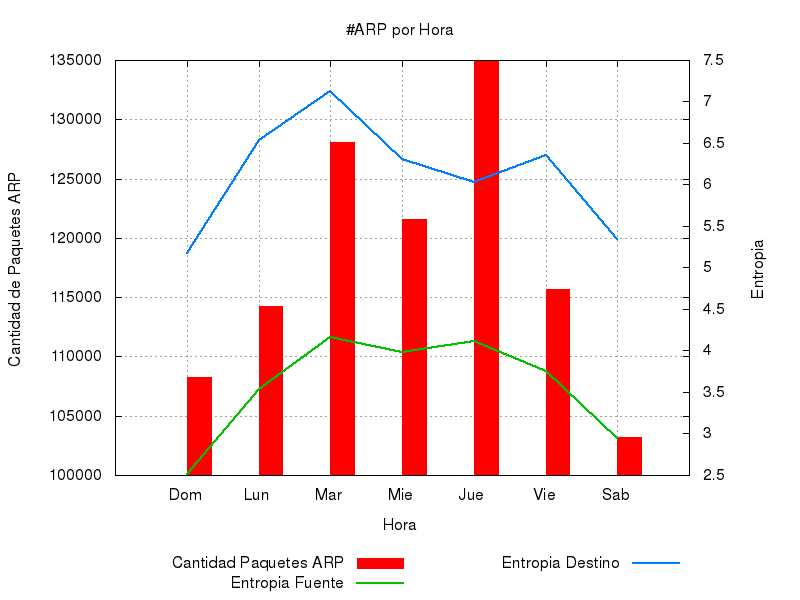
\includegraphics[width=0.5\textwidth]{img/graph/escenario_1/vlan10/vlan10_arp_vs_entropia}} &
        \subfloat[\nameref{itm:vlan20}]{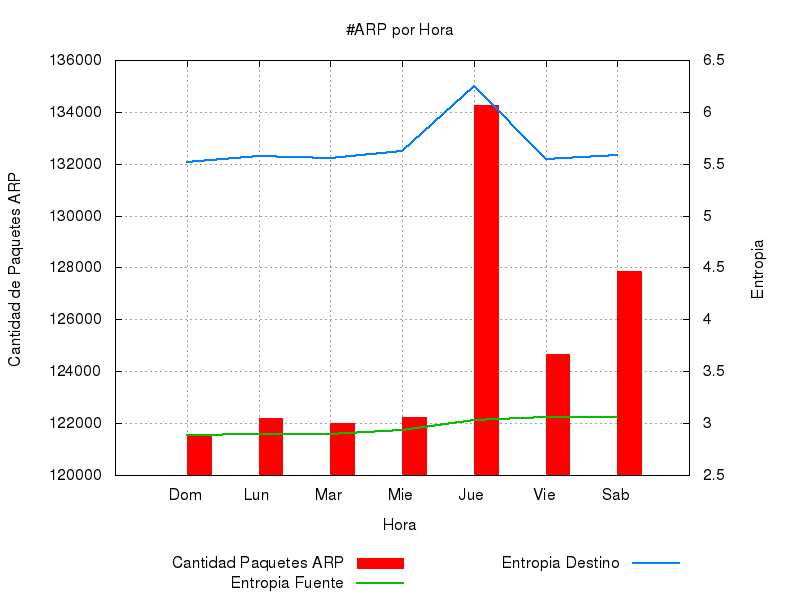
\includegraphics[width=0.5\textwidth]{img/graph/escenario_1/vlan20/vlan20_arp_vs_entropia}} \\
        \subfloat[\nameref{itm:vlan40}]{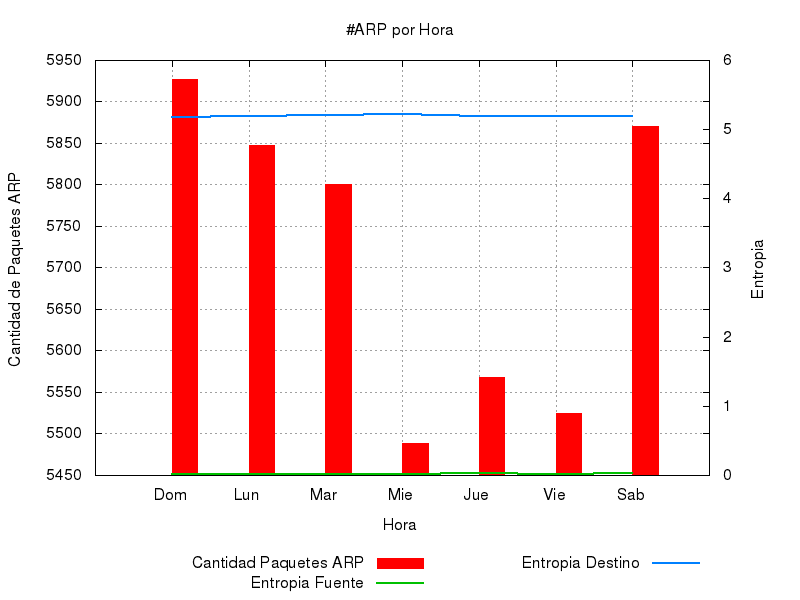
\includegraphics[width=0.5\textwidth]{img/graph/escenario_1/vlan40/vlan40_arp_vs_entropia}} &
        \subfloat[\nameref{itm:vlan1}]{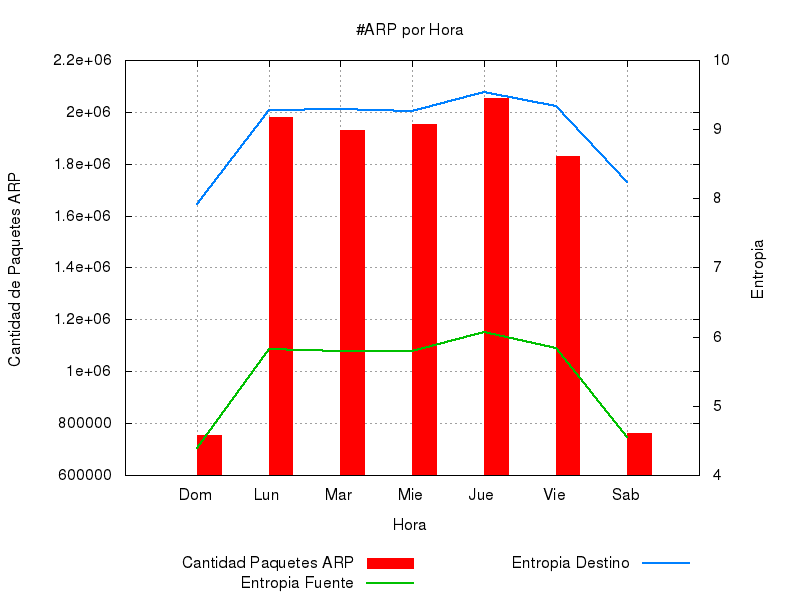
\includegraphics[width=0.5\textwidth]{img/graph/escenario_1/vlan1/vlan1_arp_vs_entropia}} \\
    \end{tabular}
    \caption{Cantidad de paquetes ARP por hora}
\end{figure*}
